\section{Zielsetzung}
Ziel des Versuches ist das Erlernen der Grundlagen der Vakuumphysik und des Umgangs mit den Komponenten der Vakuumtechnik.
Dazu wird das Saugvermögen von zwei verschiedenen Pumpen auf jeweils zwei verschiedene Arten bestimmt.

\section{Theorie}
\label{sec:Theorie}
\subsection{Definition des Vakuums}
Ein Vakuum ist definiert als ein Raum, in dem sich nur sehr wenige Teilchen befinden, sodass der Druck in disem Raum deutlich unter dem Atmosphärendruck $p_0 = \SI{1013}{mbar}$ liegt.
Je weniger Teilchen sich in einem Raum befinden, und damit je kleiner der Druck ist, desto besser ist das Vakuum.
Je nach Druckbereich wird zwischen verschiedenen Kategorien des Vakuums unterschieden. Diese sind in \autoref{tab:Vakuumtypen} aufgelistet.

\begin{table}
	\centering
	\caption{Druckbereiche in der Vakuumtechnik \cite{V070_glossar}.}
	\label{tab:Vakuumtypen}
	\begin{tabular}{| c | c |}
		%\toprule
		%{$ g\:/\: \si{cm}$} & {$ b\:/\: \si{cm}$} & {$ B\:/\: \si{cm}$} & {$ V_1$} & {$ V_2$} & {$ \lvert \Delta V \rvert$} & {$ f\:/\: \si{cm}$} \\
		\midrule
            Grobvakuum & $\SI{1}{bar}$ bis  $\SI{1}{mbar}$ \\
            Feinvakuum & $\SI{1}{mbar}$ bis  $\SI{10e-3}{mbar}$ \\
            Hochvakuum & $\SI{10e-3}{mbar}$ bis  $\SI{10e-7}{mbar}$ \\
            Ultrahochvakuum & $\SI{10e-7}{mbar}$ bis  $\SI{10e-12}{mbar}$ \\
            Extremes Ultrahochvakuum & weniger als $\SI{10e-12}{mbar}$ \\
		\bottomrule
	\end{tabular}
\end{table}

Vakuumtechnik wird in einer Vielzahl von verschiedenen Feldern eingesetzt wie beispielsweise in der Halbleiterindustrie, in der Medzin oder in der Kernforschung
im inneren von Teilchenbeschleunigern.\cite{V070_glossar}

\subsection{Physikalische Grundlagen}
\subsubsection{Druck}
Der Druck innerhalb eines Behälters ist definiert als die Kraft pro Fläche, die durch den Aufprall
der Gasmoleküle auf die Wände des Behälters ausgeübt wird. In einem Vakuum befinden sich nur wenige Moleküle, daher kann der Druck durch die ideale Gasgleichung
\begin{equation}
    \label{eq:id_gasgleichung}
    pV = N k_{\text{B}} T
\end{equation}
beschrieben werden. $p$ ist dabei der Druck, $V$ das Volumen des Behälters. $N$ ist die Teilchenzahl, $k_{\text{B}}$ die Boltzmann-Konstante und $T$ die Temperatur.
Sind Temperatur und Teilchenzahl konstant, gilt das Boyle-Mariottsche Gesetz:
\begin{equation}
    \label{eq:boyle_mariott}
    pV = \text{const.} \quad \Rightarrow \quad \frac{p_1}{p_2} = \frac{V_2}{V_1} .
\end{equation}
\cite{V070_glossar}
\subsubsection{Adsorbtion, Absorbtion, Desorption, Diffusion}
Im folgenden werden einige Prozesse beschrieben, die in der Vakuumphysik auftreten:
\begin{description}
    \item[Adsorbtion:] Prozess, bei dem Gasmoleküle an der Oberfläche eines Körpers haften bleiben.
    \item[Absorbtion:] Prozess, bei dem Teilchen in einen Festkörper eindringen und dort gelöst oder verteilt werden.
    \item[Desorption:] Umkehrprozess zur Adsorbtion. Teilchen, die an der Oberfläche haften, lösen sich von dieser.
    \item[Diffusion:] Prozess, bei dem sich Teilchen aufgrund von Konzentrationsunterschieden bewegen.
\end{description}
\cite{V070_glossar}
\subsubsection{Strömungsarten}
Anhand ihres Fließverhaltens und daran, welche Wechselwirkungen die Teilchen ausüben wird zwischen verschiedenen Strömungsarten unterschieden:
\begin{description}
    \item[Laminare Strömung:] Die Teilchen bewegen sich in parallelen Schichten, die einzelnen Schichten gleiten dabei übereinander ohne sich zu verwirbeln.
    Die Moleküle wechselwirken hauptsächlich miteinander.
    Sie ist charakterisiert durch eine Reynoldszahl $\text{Re} < 2300$ und tritt vorwiegend im Grobvakuum auf.
    \item[Turbulente Strömung:] Die Teilchen bewegen sich chaotisch, es kommt zu Verwirbelungen innerhalb der Strömung. Die turbulente Strömung ist charakterisiert
    durch eine Reynoldszahl $\text{Re} > 4000$, sie tritt im Grobvakuum oder bei hohem Druck auf.
    \item[Knudsen-Strömung:] Die mittlere freie Weglänge der Teilchen ist verglecihbar mit den räumlichen Dimensionen des Systems. Die Moleküle wechselwirken daher sowohl miteinander
    als auch mit der Wand des Systems. Die Strömung wird charakterisiert durch die Knudsen-Zahl $\text{Kn} < \lambda / L$, dabei ist $\lambda$ die mittlere freie Weglänge der Moleküle
    und $L$ eine charakteristische Länge des Systems. Die Knudsen-Zahl liegt bei der Knudsen-Strömung zwischen $0.1$ und $10$.
    \item[Molekulare Strömung:] Bei der molekularen Strömung sind nur noch wenige Moleküle im System. Die Moleküle wechselwirken fas ausschließlich mit der Wand des Systems, 
    Wechselwirkungen untereinander sind selten. Die Strömung wird charakterisiert durch eine Knudsen-Zahl $\text{Kn} > 10$ und tritt im Hoch- und Ultrahochvakuum auf.
\end{description}
\cite{V070_glossar}
\subsection{Funktionsweise einer Vakuumpumpe}
\subsubsection{Drehschieberpumpe}
\begin{figure}
    \centering
    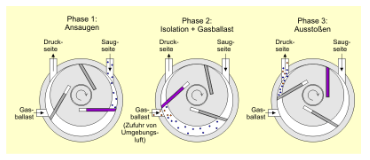
\includegraphics{content/DP.PNG}
    \caption{Funktionsweise der Drehschieberpumpe \cite{V070_glossar}.}
    \label{fig:Drehschieberpumpe}
  \end{figure}
Die Drehschieberpumpe besteht im Wesentlichem aus einem Hohlzylinder in dem eine exzentrische gelagerter Rotor angebracht ist (siehe \autoref{fig:Drehschieberpumpe}).
In den Rotor sind Schieber eingelassen, die durch Federn oder Fliehkraft gegen die Gehäusewand drücken. Bei Rotation des Rotors ensteht an der Saugseite ein Hohlraum, dessen Volumen
kontinuierlich vergrößert wird. Nach dem Boyle-Mariottschen Gesetz (Gl. \eqref{eq:boyle_mariott}) wird bei steigendem Volumen der Druck kleiner. Hat der Hohlraum sein maximales
Volumen erreicht, wird dieser durch den nächsten Schieber isoliert und über das Auslassventil ausgestoßen. Durch kontinuierliches Wiederholen dieses Prozesses kann der Druck im
Rezipienten reduziert werden \cite{V070_glossar}. Die Drehschieberpumpe kann Enddrücke von etwa $\SI{10e-3}{mabr}$ erreichen.\cite{cern_vacuum}
\subsubsection{Turbomolekularpumpe}
Die Turbomolekularpumpe, oder auch Turbopumpe, besteht im Wesentlichen aus einer Anordnung von Rotor- und Statorscheiben, welche abwechselnd im Gehäuse angeordnet sind.
Trifft ein Gasatom auf eines der rotierenden Rotorblätter, wird es in Richtung des Pumpenausgangs beschleunigt. Trifft es auf ein Statorblatt, wird es in Richtung des nächsten Rotorblattes
abgelenkt. Durch diese Anordnung entsteht eine bevorzugte Bewegungsrichtung zum Pumpenausgang bei den Molekülen. Zu beachten ist dabei, dass die Turbopumpe nur bei molekularer
Strömung effizient arbeitet, da andernfalls die Impulse der Moleküle bei Stößen untereinander wieder in beliebige Richtungen gestreut werden. Daher wird in der Regel eine
Vorpumpe genutzt, die den Druck zuvor auf einen geeigneten Wert absenkt \cite{V070_glossar}. Mit der Turbomolekularpumpe können Drücke im Bereich des Ultrahochvakuums erreicht werden.\cite{cern_vacuum}

\subsection{Saugvermögen einer Vakuumpumpe}
Eine wichtige Kenngröße einer Vakuumpumpe ist das Saugvermögen.
Durch die Pumpe entsteht ein Teilchenstrom $I_T = dN/dt$ über den Moleküle aus dem Rezipienten abtransportiert werden.
Wird die Teilchendichte $n = N/V$ eingesetzt ergibt sich
\begin{equation}
    I_T = n \frac{dV}{dt} .
\end{equation}
Mit der idealen Gasgleichung \eqref{eq:id_gasgleichung} ergibt sich daraus
\begin{align}
    I_T &= \frac{p}{k_B T} \frac{dV}{dt} \\
    \Leftrightarrow I &= I_T k_B T = p \frac{dV}{dt} = p S(p) .
\end{align}
$S(p) = dV/dt$ ist dabei der Volumendurrchsatz oder das Saugvermögen der Pumpe, $I$ beschreibt den Gasmengendurchsatz oder die Saugleistung.\cite{V070_glossar}

\subsubsection{Leitwert}
In der Realität steht nicht das gesamte Saugvermögen der Pumpe zur Verfügung, es wird durch den Aufbau der Anlage verringert.
Eine Kenngröße für die Fähigkeit eines Bauteils Gasmoleküle zu transportieren ist der Leitwert $C$:
\begin{equation}
    C =\frac{1}{W} = \frac{\dot V}{\Delta p} ,
\end{equation}
dabei ist $W$ der Strömungswiderstand des Bauteils, $\dot V$ der effektive Volumenstrom der durch das Bauteil transportiert wird und $Delta p$ der Druckunterschied zwischen den beiden
Enden.
Der Leitwert ist im wesentlichen abhängig von der Geometrie des Bauteils, dem Druckbereich sowie von der Art des genutzten Gases.
Das effektive Saugvermögen $S_\text{eff}$ lässt sich aus dem Nennsaugvermögen $S_0$ und dem Leitwert bestimmen nach
\begin{equation}
    \label{eq:leitwert}
    \frac{1}{S_\text{eff}} = \frac{1}{S_0} + \frac{1}{C} \quad \Rightarrow S_\text{eff} = \frac{S_0 C}{S_0 +C} .
\end{equation}
\cite{V070_glossar}
\subsubsection{Evakuierungskurve eines Vakuumsystems}
Eine wichtiges Werkzeug das Saugvermögen eines Systems zu bestimmen ist die Evakierungskurve. Dabei wird der Verlauf des Druckes $p$ innerhalb des Rezipienten
gegen die zeit $t$, üblicherweise logarithmisch, aufgetragen. Am Graphen lassen sich dann in der Regel verschiedene Bereiche identifizieren:
In der Anfangsphase sinkt der Druck schnell ab. Nach einiger Zeit flacht die Kurve ab, in dieser Übergangsphase verlangsamt sich der Druckabfall.
In der nächsten Phase flacht die Kurve noch weiter ab. Die Effektivität der Pumpe wird durch Leckagen oder Desorptinsprozesse begrenzt, es stellt sich ein annähernd konstanter Enddruck ein.
Ein mathematischer Ausdruck für die Evakierungskurve kann gefunden werden, indem die Gleichung des Boyle-Mariottschen Gesetzes nach der Zeit abgeleitet wird:
\begin{equation}
    \frac{d(pV)}{dt} = 0  \quad \Rightarrow  p \frac{dV}{dt}  + V \frac{dp}{dt} = 0 .
\end{equation}
Durch Einsetzen des Saugvermögens $S = dV/dt$ ergibt sich die Differentialgleichung
\begin{equation}
    \frac{d(p)}{dt} = - \frac{S}{V} \cdot p = 0 .
\end{equation}
Die Differentialgleichung wird gelöst durch
\begin{equation}
    p(t) = p_0 \exp\left(- \frac{S}{V} \cdot t \right) + c.
\end{equation}
$p_0$ ist dabei der Startdruck. Da Vakuumpumpen ein endliches Saugvermögen besitzen, wird der Enddruck $p_E$ eingeführt.
Dadurch wird die vorherige Gleichung zu
\begin{equation}
    \label{eq:evakuierung}
    p(t) = (p_0 - p_E) \exp\left(- \frac{S}{V} \cdot t \right) + p_E \quad \Rightarrow \ln \left(\frac{p(t) - p_e}{p_0 - p_E}\right) = - \frac{S}{V} \cdot t
\end{equation}
korrigiert. Zu beachten ist dabei, dass in dieser Rechnung das Saugvermögen als unabhängig vom Druck betrachtet wurde.
In der Praxis kann dieses allerdings stark vom Druck abhängig sein.\cite{V070_glossar}

\subsubsection{Lecks und Leckraten}
Der Enddruck eines Vakuumsystems ist begrenzt durch auftretende Leckagen, durch welche Gas in das System eintreten kann.
Es wird im Allgemeinen zwische realen und virtuellen Lecks unterschieden. Ein reales Leck ist eine physische Öffnung im System, durch welche Gas von außen
eindringt. Diese werden beispielsweise durch poröse Materialien oder defekte Dichtungen erzeugt.
Bei virtuellen Lecks dagegen tritt das gas nicht von außen, sondern aus inneren Hohlräumen, beispielsweise aus in Kammern eingeschlossener Luft oder durch Desorptionsprozesse,
in das System ein.
Die Leckrate wird definiert nach
\begin{equation}
    Q_\text{Leck} = p \dot V ,
\end{equation}
dabei ist $p$ der Druck des eindringenden Gases und $\dot{V}$ dessen Volumenstrom.

Durch kontrolliertes Einfügen eines Lecks in ein Vakuumsystem kann durch eine Druckanstiegsmessung das Saugvermögen der Pumpe bestimmt werden.
Dazu wird bei laufender Pumpe ein reales, einstellbares Leck, beispielsweise durch ein Justierventil, in das System gebracht.
Es stellt sich ein konstanter Gleichgewichtsdruck $p_g$ ein. In diesem Fall gilt dann
\begin{equation}
    Q_\text{Leck} = S_\text{eff} p_g ,
\end{equation}
mit dem effektivem Saugvermögen $S_\text{eff}$.
Wird nun die Pumpe über ein Ventil abgeklemmt, steigt der Druck im Rezipienten. Die Leckrate kann durch Beobachtung des Druckanstiegs bestimmt werden zu
\begin{equation}
    \label{eq:Leckrate}
    Q_\text{Leck} = V \frac{\Delta p }{\Delta t} .
\end{equation}
$V$ ist dabei das Volumen des Rezipienten, $\frac{\Delta p }{\Delta t}$ die Druckanstiegsrate.
Durch Gleichsetzen der beiden Gleichungen lässt sich ein Audruck für das Saugvermögen aufstellen:
\begin{equation}
    \label{eq:s_leck}
    S_\text{eff} = \frac{V}{p_g} \frac{\Delta p }{\Delta t} . 
\end{equation}
\cite{V070_glossar}